\chapter{Cosmological Considerations}

\begin{doublespace}

\section{A Brief History of Cosmology}

Cosmology is one of the oldest and perhaps the grandest of human sciences.
The word \char`\"{}cosmos\char`\"{} is commonly understood to represent
the entire Universe. It originates from the Greek word for order i.e.
the opposite of chaos and disorder \cite{Wikipedia2008Cosmology}. Since
ancient times, across history and all civilizations the human mind
has always been drawn to the night sky and to the order apparent in
it. What, our curiosity compels us to ask, is the mechanism that causes
this Order to come about, not only in our planetary sphere but on
the scale of the stars and galaxies? Today the word {}``cosmology''
has a somewhat narrower interpretation in terms of the study of the
dynamics of the Universe in the language of physics and mathematics,
but though the language might have become more structured the essential
question remains the same.

The first viable mathematical description of a cosmological model
was possible only after the discovery of General Relativity by Albert
Einstein\cite{Einstein:1920RelativityBook}, a framework which allows
us to describe the motion not only of matter but also of the spacetime
manifold in which matter lives. Even though Einstein himself, for
personal and aesthetic reasons, was a proponent of a static universe,
the discovery of solutions for expanding cosmological metrics by DeSitter,
Freidmann, Le'Maitre and others pointed elsewhere. The discovery of
the redshifting of the spectra of distant nebulae and galaxies by
Edwin Hubble in 1920\cite{Hubble:1929PNAS} provided concrete evidence
for an expanding universe. This discovery raised even more vexing
questions. If the Universe is expanding in the present epoch then
at some earlier epoch all the matter and energy must have existed
in the form of an incredibly dense and hot Cosmic egg. This birthing
scenario for the Universe came to be known as the {}``Big Bang''
hypothesis. At this stage not only gravitational but also quantum
mechanical fluctuations would become significant. Thus a theory of
{}``quantum gravity'' would necessarily be required to properly
describe the earliest epoch of the Universe. Consequently research
in theoretical cosmology since the 1930s until the present has essentially
been a quest for such a unification of the two pillars of modern physics:
Quantum Mechanics and General Relativity.

The lack of a complete understanding of such a unification becomes
stark when considering one of the key elements of General Relativity
as formulated by Einstein - the Cosmological Constant (CC). Einstein
originally introduced this parameter into his field equations in order
to obtain a static cosmological solution which as mentioned above
seemed most natural to him. Including this term the field equations
become \cite{Wald1984General}:

\begin{equation}
G_{\mu\nu}=8\pi G\; T_{\mu\nu}-\Lambda\: g_{\mu\nu}\label{eq:GRFieldEqn}
\end{equation}


where $G_{\mu\nu}$ is the Einstein tensor, $T_{\mu\nu}$ is the matter
stress-energy tensor, $g_{\mu\nu}$ is the metric tensor and $\Lambda$
is the CC. Now the simplest form for $T_{\mu\nu}$ is that of a perfect
fluid:

\begin{equation}
T_{\mu\nu}=\rho u_{\mu}u_{\nu}+p(g_{\mu\nu}+u_{\mu}u_{\nu})\label{eq:PerfectFluidTensor}\end{equation}


where $\rho$, $P$ are the density and pressure, respectively, of
the fluid w.r.t an (unaccelerated) observer whose trajectory is given
by the four-vector $u_{\mu}$. With the CC term the effective stress-energy
tensor becomes:

\begin{equation}
T_{\mu\nu}=(\rho+p)u_{\mu}u_{\nu}+(p-\frac{\Lambda}{8\pi G})g_{\mu\nu}\end{equation}


or more explicitly for a stationary observer whose trajectory is given
by $u_{\mu}=(-1,0,0,0)$ in a flat background with metric $g_{\mu\nu}=diag(-1,1,1,1)$:

\begin{equation}
T_{\mu\nu}=\left(\begin{array}{cccc}
\rho+\frac{\Lambda}{8\pi G}\\
 & p-\frac{\Lambda}{8\pi G}\\
 &  & p-\frac{\Lambda}{8\pi G}\\
 &  &  & p-\frac{\Lambda}{8\pi G}\end{array}\right)\end{equation}


from which we can see that the CC term behaves as a perfect fluid
with energy density $\frac{\Lambda}{8\pi G}$ and \emph{negative}
pressure $-\frac{\Lambda}{8\pi G}$. This behavior is also characterized
by the \emph{equation of state}:

\begin{equation}
w=\frac{p}{\rho}\end{equation}


In the absence of any other forms of matter we have $\rho=\frac{\Lambda}{8\pi G}$
and $p=-\frac{\Lambda}{8\pi G}$, giving $w=-1$. Thus any form of
matter which has equation of state $w=-1$ has the same physical effect
on cosmological dynamics as the CC term.

For a metric parametrized by a scale factor $a(t)$ and the parameter
$k$, which takes on values $-1,0,1$ corresponding to an open (hyperbolic),
flat and closed ($S^{3}$) spatial topologies respectively:

\begin{equation}
ds^{2}=-dt^{2}+a^{2}(t)\left[ \frac{dr^{2}}{1-kr^{2}}+r^{2}(d\theta^{2}+sin^{2}(\theta)d\phi^{2}) \right]\end{equation}


and the stress-energy tensor of a perfect fluid with a CC term, only
the diagonal components of the Einstein tensor are non-zero and the
field equations reduce to \cite{Wald1984General}:

\begin{eqnarray}\label{eqn:Friedmann}
\frac{\dot{a^{2}}}{a^{2}} & = &\frac{8\pi G\rho}{3}+\frac{\Lambda}{3}-\frac{k}{a^{2}} \\
\frac{\ddot{a}}{a} & = & -\frac{4\pi G}{3}(\rho+3p-\frac{\Lambda}{4\pi G})
\end{eqnarray}


which are referred to as the first and second Friedmann equations
respectively. We can see from the first equation that for $k=+1$,
there exists a $\Lambda>0$ such that the $H^{2}=\frac{\dot{a^{2}}}{a^{2}}=0$.
For a suitable value of $p$, we can also set the RHS of the 2nd equation
to zero. This solution is known as the Einstein-static universe. It
is clear that without the presence of the CC term in the 2nd term
such a static solution would not be possible. It is an easy exercise
to show that this solution is unstable w.r.t small perturbations in
the scale factor. Therefore the Einstein-static universe, apart from
being in conflict with observation is also not a mathematically stable
solution. Thus Einstein's introduction of the CC term was a failure
in that it cannot be used to obtain a stable static solution. Subsequently
Einstein would refer to the CC term as his {}``greatest blunder''%
\footnote{Even in this {}``blunder'', Einstein had discovered a term that
lies at the crux of the clash between GR and QM and continues until
today to vex theorists and experimentalists alike with its resistance
to a final satisfactory resolution as to its physical origins and
significance.%
}.

As the focus of cosmological research moved on to the study of special
solutions of (\ref{eq:GRFieldEqn}) describing stars and black holes,
the realization of the true significance of this cosmological term
was postponed until the last decade of the 20 century when enough
evidence had accumulated from cosmological observations involving
ground and space-based platforms examples and references HST, COBE etc. to rule out all cosmological models except those with non-zero $\Lambda$ \cite{Spergel2006Wilkinson}

\subsection{Problems with FRW Models}

Though Hubble's discovery provided confirmation that the large scale structure of the cosmos was amenable to a description within the framework of Einstein's General Relativity, this was merely the beginning of the story. It was clear that the observable universe contained a great deal of structure and that any cosmological model would be considered incomplete if it did not provide some explanation as to how these large-scale inhomogeneities could form. A further layer of confusion was added by Penzias and Wilson's discovery \cite{Penzias1965A-Measurement} of the cosmic microwave background (CMB) radiation which appeared to be isotropic and uniform at a temperature of $\sim 3^{\circ}$ K, with negligible fluctuations. This radiation was the imprint of the recombination era, the time when the universe had cooled enough for electrons and protons to form hydrogen atoms. Naturally any gravitational inhomogeneities present at that epoch would have left a signature on the radiation emitted during recombination. And these same inhomogeneities constituted the seeds of present day large scale structure. However a simple calculation assuming a FRW cosmological model, shows that the structures which lie within our Hubble horizon ($\sim 3000 \, Mpc \sim 10^{26} m$) could not have been in causal contact at $t_{rec}$. How could one reconcile this observation with the observed isotropy and homogeneity of the CMB? We also happen to live in a universe with a predominance of matter over anti-matter.\footnote{The alternative would clearly be unsuitable not only for life but for any kind of stable structures such as planets and galaxies.} Now the Standard Model description of elementary particles does not incorporate CP violation, which would be required for one form of matter to be predominant. What mechanism could explain this matter-antimatter asymmetry?

\subsection{Inflationary Cosmology}

In 1982 Alan Guth, and Vilenkin and Starobinsky in the following year, proposed a new paradigm for the early universe: the inflationary model. The elegance of this solution lay in the fact that it had the potential to explain all three of the above problems (horizon/flatness problem, structure formation and matter-antimatter asymmetry) in one stroke. The idea behind inflation is simple enough. As the word implies, the universe underwent a period of exponential growth when the scale factor $a(t)$ grew as $\sim e^{-H_{inf} t}$ ($H_{inf}$ is the Hubble rate during this era) starting from some small homogenous, isotropic patch of geometry. This rapid expansion would damp out any large scale geometrical inhomogeneities present prior to inflation, avoiding the need to fine-tune the matter density at early epochs, and would naturally yield the flat, isotropic background as characterized by the CMB, leaving only small density fluctuations whose amplitude ($\delta \rho/\rho \sim 10^{-5}$) depends only on the duration of the inflationary phase. Being a non-equilibrium process, inflation provides the conditions necessary for CP violating processes to occur, which would then naturally yield an excess of particles over anti-particles.

Despite these attractive features, the biggest obstacle to accepting the validity of this model was the lack of a sensible physical mechanism. Guth's original proposal was that of \emph{false vacuum decay}. The initial state of geometry is described by a quantum state that is trapped in the false minimum of a potential. As the temperature falls, the potential is lowered sufficiently to allow the state to tunnel out resulting in bubbles of inflationary patches to grow. This model however ran into trouble because the speed of expansion of these bubbles was insufficient to allow them to combine and reach equlibrium, resulting in a highly inhomogenous universe at the end of the inflationary phase, in conflict with the homogeneity of the CMB. The other most commonly adopted class of models was based on the notion of "slow-roll". A scalar field can be shown to have a negative equation of state, the same as a positive cosmological constant and can thus drive inflation. In order to obtain the required duration of inflation, followed by a period of reheating, the potential for this scalar would in general have to have a very specific form determined by the so-called "slow-roll" conditions. The ad-hoc nature of this potential and the lack of a suitable scalar field in the Standard Model are the main deficiencies of this class of models\footnote{The SM is posited to contain the U(1) Higgs axion which is supposed to endow particles with mass via a sponatenous symmetry breaking mechanism. It is unclear however if the Higgs would correspond to the inflaton and if so how could they be related.}. In recent years, alternatives to inflation such as the ekpyrotic and bouncing universe scenarios have been proposed. String Theory has also provided fertile ground for alternatives to inflation such as the brane collision model \cite{Khoury2001Physical}. However, none of these alternatives has the simplicity and elegance of the inflationary scenario. The question then arises: can we come up with some mechanism which generates inflation without resorting to ad-hoc potentials or exotic scalar/quintessence fields which \emph{a priori} don't have sufficient grounding in our (reasonably complete) picture of the Standard Model of particles?

In this thesis, we argue that a cosmological condensate which forms via the BCS mechanism can source inflation without resort to ad-hoc potentials and also provide a resolution to the cosmological constant problem. Venturing into the speculative realm, we also conjecture that such an axion would play the role of the Higgs scalar. Inflation has the character of a phase transition. Phase transitions in particle physics are generally understood within the framework of \emph{spontaneous symmetry breaking} (SSB). An axion with U(1) symmetry could undergo SSB and be responsible for both driving inflation and endowing leptons with mass, thus playing the role of the inflaton + Higgs.

\section{Many-Body Phenomena and Gravity}

Physics has come a long way from the days of the Newtonian point particle and exactly solvable two-body systems. It is now clear that it is \emph{many body} phenomena than constitute the phenomena in Nature of deepest interest to us. Some examples of such theories are

\begin{itemize}
\item fluid-flow or hydrodynamics, under whose coarse-grained banner falls everything from the sloshing of tea in a cup to oceanic and atmospheric currents.
\item condensed matter, hard and soft, encompasses the behaviour of systems with electronic energy band structures; fermi and non-fermi liquids; excitons, polarons and other excitations in crystalline media.
\item quantum field theory, which seeks to describe the behaviour and interactions of elementary particles and gauge fields which ultimately determine the nature of the strong and electroweak forces the glue holding nuclear structure together.
\end{itemize}

In light of the arena of gravitational physics, ranging from planetary systems to galaxies, one might be tempted to think of general relativity as also being a many body phenomena. Indeed the equations of GR describe the interaction of \emph{fields} of matter and geometry, which like all fields are continuum descriptions of an underlying many body theory. However, even though the many body nature of gravitation is implicit in the structures used to define it, most physicists would initially balk at such a description.

\subsection{The Cosmological Constant term in Field Theory}

While the most concrete evidence for a non-zero $\Lambda$ has come from astronomical observations, one can also investigate this question from the perspective of local QFT and/or candidates for theories of Quantum Gravity (QG) such as LQG and String Theory. But first, let us consider the simple case of the quantum harmonic oscillator.

One of the most striking results of early quantum mechanics was Dirac's quantization of the harmonic oscillator hamiltonian is the energy eigenstate basis. The resulting hamiltonian becomes:

\begin{equation}
\hat{H} =  \hbar \omega \sum_{\vec{k}} \left( a^\dagger_{\vec{k}} a_{\vec{k}}  + \frac{1}{2} \right)
\end{equation}

where $\omega$ is the characteristic frequency of the given oscillator. This expression might seem passe to most physicists, having encountered it one too many times in the literature. However, let's rewrite it as:

\begin{equation}
\hat{H} = \hat{H}_{kin} + \hat{H}_{\Lambda} = \left( \hbar \omega \sum_{\vec{k}} a^\dagger_{\vec{k}} a_{\vec{k}} \right) + \left( \sum_{\vec{k}} \frac{1}{2} \hbar \omega \right)
\end{equation}

It is clear that the second term $\hat{H}_\Lambda $ is a divergent sum, at least for a free harmonic oscillator. This is referred to as the \emph{zero-point energy} and arises due to the commutation relations of the ladder operators. Its presence clearly indicates a difficulty. The ground state of a SHO is characterised by a divergent energy term. In practice, this term is considered a minor annoyance as in any physical observation it is the energy \emph{difference} between two states that is measured, and can therefore be ignored for all practical purposes (FAPP). This is no longer the case when gravity is included in the picture. These "zero-point" fluctuations will now contribute to the expectation value $\expect{T_{\mu\nu}}$ of the stress-energy tensor and hence lead to metric perturbations which can no longer be neglected. In general, due to the interaction of matter and geometry as codified by the equivalence principle, any matter fields will receive some non-zero correction to their self-energy in a given background metric. In principle this is a good thing. It should regulate the divergent sums as found above in $\hat H_\Lambda$ by modifying the dispersion relation at high momenta.

What we refer to as the cosmological constant from the perspective of QFT is precisely the zero-point contribution to the vacuum energy from all Standard Model matter fields. This contribution ($\hat H_{SM}$) would constitute the $T_{00}$ term of the vacuum stress-energy tensor and the solution of the Einstein equations is deSitter spacetime with $\Lambda_{SM} = \expect{\hat H_{SM}}$. $\Lambda_{SM}$ would also act as a natural momentum cutoff for integrals in the SM.

So far we have not encountered any contradictions. Matter quantum fields have a divergent zero-point energy. This energy should play the role of a positive $\Lambda$ when gravity is included in the picture and should act as a momentum cut-off thereby regulating divergences in the field theory. Seen this way, gravity is nature's way of keeping vacuum fluctuations in check \cite{Crane1985Space-time}.

However, the ratio of the CC as obtained from WMAP3 and other cosmological observations ($\Lambda_{obs}$) happens to be smaller than that calculated from SM fields ($\Lambda_{SM}$) by a factor of about $10^{-120}$. What is the explanation for this massive discrepancy? Regardless of its origin, this number points to a lack of knowledge about the SM and/or a quantum theory of gravity. In the 1960s, theorists realized that the mechanism of supersymmetry could alleviate the problem somewhat. In this picture every SM particle has a supersymmetric dual whose vacuum fluctuations are of opposite sign as those of the original particle. This leads to a partial cancellation when computing $\Lambda_{SM}$. The magnitude of the problem is then reduced but the ratio $\Lambda_{obs} / \Lambda_{SM}$ still remains a gargantuan $10^{-60}$. Also the inclusion of SUSY raises more questions. Since we don't observe SUSY particles in nature and none have so far been found in high energy experiments\footnote{Though it is believed that the spectrum of high energy cosmic rays might be due to decaying relic SUSY particles}, we need a mechanism to break SUSY at some point before the radiation era. Also if SUSY is broken then it is hard to see how it could effect the CC problem in the present epoch. By itself, SUSY is another beautiful symmetry of nature and will likely be observed at some point either in the LHC or perhaps in the realm of condensed matter physics.\footnote{This is, of course, a very simplified summary of the actual picture. In QFT $\expect{H_{SM}}$ corresponds to the one-loop energies of all the possible SM interaction vertices. However, the physical essence of the reasoning presented above remains the same.}

Insert para about how it is $G_{N}^{2} \Lambda_{SM}$ and not $G_{N}$ which determines the strength of the coupling between matter fields and gravity. As it so happens, in the proper units, $G_{N}^{2} \Lambda_{SM} \sim 10^{120} \Lambda_{obs}$. How does this factor into the picture ???

Of course, one might ask if it even makes sense to compare two quantities associated with vastly different scales: $\Lambda_{SM}$ corresponding to the scale of electroweak theory ($\sim 10^{-15} m$) and $\Lambda_{obs}$ corresponding to the scale of CMB horizon ($\sim 10^{26} m$). Assuming that the large-scale structure of geometry can be described by a condensate, such a comparison becomes essentially meaningless. We know from our knowledge of many-body physics that fluctuations above the correlation length of a condensate are strongly suppressed relative to microscopic scales. If we wish to adopt this perspective, then we must explain how such a condensate can form and how its correlation length comes to exceed the range of the weak force. One might speculate that given a reasonably complete picture of condensate formation the second question might be answered naturally. In this thesis, we outline the first steps towards such a complete picture.

\subsection{Elements of LQG}

There are two principle approaches to the problem of reconciling gravitational physics with quantum theory. The first is String Theory (ST) which is founded around the study of excitations of extended objects - strings and higher dimensional branes - embedded in a flat spacetime. The second is Loop Quantum Gravity (LQG) which attacks the problem from a different perspective, one that seeks to preserve the principle feature of general relativity - background independence. Here the notion is that by quantizing around a flat background - as is done in String Theory - we sacrifice background independence and then there is no guarantee that the resulting theory can correctly describe the quantum fluctuations of geometry especially in the strong-field regime.

The principle obstacle to covariant quantization approaches was the non-renormalizability of the gravitational action, a problem rendered even more difficult due to its non-quadratic form. The Einstein-Hilbert action is:

\begin{equation}\label{eqn:EinsteinHilbert}
	S_{EH} = \int d^{4}x \sqrt{-g} \, \mathcal{R}
\end{equation}

where $\mathcal{R}$ is the Ricci scalar and $g$ is the determinant of the metric element. One can see that due to the non-polynomial nature of this action, because of the presence of the $ \sqrt{-g} $, the direct application of methods of QFT is not possible.

Loop Quantum Gravity (LQG) presents a fundamentally different approach
- as compared to QFT and String Theory - to the old problem of the
construction of a quantum theory of gravity. It is built upon the
recognition that via a change of variables, the action of canonical
General Relativity (GR) can be cast in a form which resembles that
of gauge theories such as Maxwell and Yang-Mills. Despite the great power and elegance of this formalism it is not yet
very widely used, due in part to the lack of accessible introductory
reviews. The concepts that arise in LQG should be familiar to anyone
acquainted with gauge theories, although the notation used can often
seem unfamiliar at first glance.

In its gauge theory-like form, the fundamental variables of GR are
no longer the metric and Christoffel connection, but a Lie-algebra
valued gauge connection $A_{\mu}^{I}$ and an orthonormal basis $\{e_{I}^{\mu}\}$
for a local frame (often called a vierbein). The great advantage of
these variables over the traditional ones is that the gauge symmetries
which encode frame-rotation are no longer obscured. Also the presence
of the gauge connection allows us to transparently include fermions
in any action via the covariant derivative with respect to the gauge
connection:\[
\mathcal{D}_{\mu}\Psi=\partial_{\mu}\Psi-gA_{\mu}^{I}T_{I}\Psi\]


where $\{T_{I}\}$ are the generators of the Lie algebra of the corresponding
Lie group, and $g$ measures the strength of the gauge coupling. In
this language GR has the same phase space as Yang-Mills theory, allowing
us to apply the powerful mathematical techniques and physical insights
of lattice gauge theory to the problem of quantum gravity.

But apart from its relevance for quantum gravity, and perhaps more importantly, such a change of language allows us a more accessible path into general relativity than the traditional foundation build around the metric tensor and its derivatives.

\subsection{Gravitation as a Many-Body Phenomenon - A concrete example}

In this thesis we show how a fermionic gas in a time-dependent background can undergo condensation and the resulting condensate can be used to generate inflation. Now, while this approach utilizes the notions of many-body physics in a gravitational background, it does not directly address the question of whether gravitation itself is best understood as many-body phenomena. A detailed analysis of this assertion is done in other work. Here we briefly outline the physical motivations for making such a claim.

The simplest physical models of inflation rely on the deSitter metric:

\begin{eqnarray}\label{eqn:deSitterMetric}
	ds^{2} & = & dt^{2} - a(t)^{2} d\mathbf{r}^{2} \nonumber \\
	           & = & \frac{1}{H_{0}^{2}\eta^{2}} ( d \eta^{2} - d \mathbf{r}^{2} )
\end{eqnarray} 

where $a^{-1}(\eta) = H_{0}\eta$ [check and fix details ...] and $\eta \in [-\infty,0]$. In these models the gravitational background is taken as a given in terms of some prescribed metric such as in \ref{eqn:deSitterMetric} or some version thereof, coupled to some matter field $\phi$\;\footnote{which satisfies the negative energy equation of state: $w=-1$} with a potential $V(\phi)$. The search for viable models of inflation has generally involved finding good candidates for the matter fields and the corresponding potentials. Any such model of inflation will necessarily be only a poor approximation to a more complete picture of quantum gravity where matter and gravitational degrees of freedom are treated in a unified manner.

In these approaches to inflation one fundamental aspect of general relativity is ignored - that gravity describes a system with precisely two degrees of freedom at each point of space-time. This is most easily via the ADM formulation of GR wherein we find that Einstein's equations can be expressed as a sum of constraints. The Ricci curvature tensor $R_{\mu\nu}$ in D dimensions has $N=(D-2)(D-1)/2$ (see Appendix 2 of \cite{Wald1984General}) degrees of freedom. For D=4, this yields N=6. We have four constraint equations (one from the scalar and three from the diffeomorphism constraint) giving us two free degrees of freedom at each point of a 3+1 dimensional background. In light of this observation the picture that comes to mind is that of a spin-system such as those encountered in condensed matter models. If we were to proceed under the assumption that such an analogy has more than merely formal content, then one can immediately export the tremendous insights gained from condensed matter physics to the gravitational arena.

In such a framework the gravitational variables such as the scale factor $a(t)$ and the corresponding conjugate momenta $\dot a(t)$ are best understood as coarse-grained expectation values of local operators defined on the spin-system, in the same manner as the magnetization in the Ising model corresponds to the average of the spins at all sites of the given lattice. The exponential growth of the scale factor in inflationary scenarios can then be interpreted as corresponding to the divergence of the correlation lengths of order parameters near a critical point in a spin-system. This point of view is also in concordance with the picture emerging from studies of quantum geometry where the spatial manifold is replaced by discretized structures called \emph{spin networks} whose edges are labeled by spins and vertices are labeled by so-called \emph{intertwiners} - which live in the space of linear operators $\mathcal{I} : \bigotimes\limits_{i \in [1..n]} \mathcal{H}_{j_{i}} \rightarrow \rm{C}$ where $\{j_{i}\}$ are the spin labels of the edges incident on that vertex. If one asked a condensed matter physicist what this picture reminds them of, the immediate answer would be: the Ising model !. Or one could ask a lattice QCD expert and they would remark on this model's similarity to their own work. After all the action for Yang-Mills theory - which with gauge group $SU(3)$ is used to model the strong interaction - is:

\begin{equation}
	S_{QCD} = \int dt d^{3}x\, Tr [ F_{\mu\nu}^{IJ}F^{\mu\nu \, KL} \sigma_{IJ} \sigma_{KL} ]
\end{equation}

where $\sigma_{IJ}$ are the generators of the relevant gauge group ($SU(3)$ for QCD) and $F^{IJ}_{\mu\nu}$ is the curvature of the gauge field. This action the same essential structure as the action for gravity. We elaborate with some mathematics:

Following Smolin \cite{Smolin2002Quantum}, we have for the Hamiltonian constraint for GR with positive $\Lambda$:

\begin{equation}\label{eqn:deSitterHamiltonian}
	\mathcal{H}_{deS} = \epsilon_{ijk} E^{\alpha i} \left ( F^{k}_{\alpha \beta} E^{\beta j} - \frac{\Lambda}{3}\epsilon_{\alpha \beta \gamma} E^{\beta j} E^{\gamma k} \right) = 0
\end{equation}

where $ (\alpha, \beta, \gamma) $ are the ``internal" or spin indices and $ \{ i,j,k \} $ are the spatial indices of the triads.

We would like to point the formal similarity between this equation and the hamiltonian for condensed matter systems, in particular the spin-ice model, where our degrees of freedom are spins $S_{i}$ placed at the vertices of a hexagonal lattice ${}^{\star}\mathcal{L}$. The dual $\mathcal{L}$ of this lattice is a triangular lattice. The spins can also be seen as being located on the faces of $\mathcal{L}$. This makes sense from the quantum geometry framework where the area operator of a surface is the Casimir $J^{2}$ of a system of spins $j_{i}$ labeling each point on the surface $p_{i}$ which is pierced by a loop carrying a flux of the gravitational connection. For this to work however, we must dimensionally reduce \ref{eqn:deSitterHamiltonian} which \emph{a priori} is the Hamiltonian of a system in three dimensions. This can be done by considering a foliation of the three dimensional space with two dimensional sheets. The triads can be understood to be spinor $ S^\alpha_i \tau_\alpha $ \footnote{$  \tau_\alpha $ are the Pauli matrices.} sitting on the edges of the lattice.

Let us fix a gauge in which we set one spinor $\vectb{E}^\gamma_{i=z} = \eta^{\gamma}$ to be the normal to the two dimensional surface $ \Sigma $. The other two triads $ \{ \vectb{E}^\alpha_x , \vectb{E}^\beta_y \} $ then become a spinorial basis or co-ordinatization of $ \Sigma $ as shown in \textbf{insert fig ...}. Then \ref{eqn:deSitterHamiltonian} can be written as:

\begin{eqnarray}
	\mathcal{H}_{deS} & = & \vectb{F}^{\alpha \beta} \cdot \vectb{E}_{x\alpha} \times\vectb{E}_{y\beta} - \frac{\Lambda}{3}  \vectb{E}_{z\gamma} \cdot \epsilon^{ \alpha \beta \gamma } \vectb{E}_{x\alpha} \times \vectb{E}_{y\beta} \nonumber \\
	& = & \left\lbrace \vectb{F}^{\alpha \beta} - \frac{\Lambda}{3} \epsilon^{\alpha \beta \gamma} \vectb{\eta}_\gamma \right\rbrace \cdot \vectb{A}_{\alpha \beta}
\end{eqnarray} 

where $ \vectb{F}^{\alpha \beta} \equiv \vectb{F}^{\alpha \beta}_z $ plays the role of a ``magnetic" field normal to $ \Sigma $. The first term can be thought of as the coupling between the area $ \vectb{A}_{\alpha \beta}(x,y) \equiv \vectb{E}_{x\alpha} \times \vectb{E}_{y\beta} $ of the lattice cell $ (x,y) $ on $ \Sigma $ and this magnetic field. The cross product ``$ \times $" is the familiar one from three-dimensional geometry.

The deSitter Hamiltonian $\mathcal{H}_{deS}$ can then be interpreted as being the sum of the terms corresponding to the kinetic energy and the nearest neighbor, two and three body interaction energies of spins $E^{ai}$ placed at the vertices of the hexagonal lattice (${}^{\star}\mathcal{L}$). The two and three body interaction energies are:

\begin{equation}\label{eqn:nBodyEnergy}
	\mathcal{E}_{2} = \sum F^{ab}_{ij} E^{i}_{a} E^{j}_{b}; \qquad \mathcal{E}_{3} = -\frac{\Lambda}{3} \sum \epsilon_{ijk} \epsilon^{abc} E^{i}_{a} E^{j}_{b} E^{k}_{c}
\end{equation}

where $i,j,k$ label vertices in $^{\star}\mathcal{L}$ and $a,b,c$ label the possible states of each spin variable. From the form of the above equations it is clear that the ``spins'' in this case have to live in a three-dimensional hilbert space $H_{3}$. The two-body interaction term contains the kinetic energy term which is given by:

\begin{equation}\label{eqn:kinTerm}
	E_{kin} = \frac{1}{2}\sum_{i} F^{ab}_{ii} E^{i}_{a} E^{i}_{b}
\end{equation}

The remaining components of the two-body term can be interpreted as exchange energies:

\begin{eqnarray}\label{eqn:exchTerm}
	E_{exch} & = & \sum_{i \neq j}  F^{ab}_{ij} E^{i}_{a} E^{j}_{b} \\
			    & = & \frac{1}{2} \sum_{i} \sum_{j > i} F^{ab}_{ij} \left( E^{i}_{a} E^{j}_{b} \pm E^{j}_{a} E^{i}_{b} \right )
\end{eqnarray}

where the sign in the last term determines the statistics the particles $E^{i}_{a}$ obey under exchange.

When restricted to a 2D space, in addition to fermionic and bosonic statistics we can have anyonic statistics, i.e. exchanging two identical objects can lead to a phase change of $e^{\imath \theta}$. The exchange term should then be written as:

\begin{equation*}
	^{2D}E_{exch} = \frac{1}{2} \sum_{i} \sum_{j > i} F^{ab}_{ij} \left( E^{i}_{a} E^{j}_{b} + e^{\imath \theta} E^{j}_{a} E^{i}_{b} \right )
\end{equation*}

where the anyon phase factor is included.

The above example illustrates how by treating tetrads as spinors, one can map the deSitter Hamiltonian onto a many-body system leaving us free to utilize the techniques and insights from condensed matter to understand the notion of emergent geometry.

\section{Cosmological Condensates}

This thesis is built around the assertion that the large scale geometry of the Universe, as given by metric and curvature invariants, can be understood as a condensate of some more fundamental degrees of freedom. However, this point of view runs into an old and venerable dispute in physics - that regarding the concept of ``ether".

Long before Quantum Gravity, physicists struggled to understand by what means could Maxwell's electromagnetic radiation be transmitted through seemingly empty space. After all, all other sorts of wave phenomena were known to occur in some \emph{medium} such as a fluid, solid or gas. The vacuum of space did not contain any material whose macroscopic excitations could be identified with light waves. Yet, light did exist, and it did propagate through the vacuum.

In order to get a hold on this issue, it came to be generally accepted that the vacuum is not truly empty but consists of a fluid referred to as the \emph{ether}, in which all other forms of matter - from planets to galaxies - were immersed. As is well known, Einstein's work on special relativity, understandably given its own revolutionary nature, caused grave damage to such an idea by asserting that the speed of light is the same for \emph{all} observers regardless of their motion through and with respect to the surrounding ether. Consequently the presence of an ethereal medium could not be confirmed by experiments such as the one performed by Michelson and Morley ( for an elaboration of this experiment see\ref{sec:MMExp}).

It took another eighty years of progress in our understand of physical processes before a new and more robust candidate for the ether came into being - the vacuum experienced by quasiparticles moving in a superfluid background. In the following we elaborate on this idea and its synthesis.

\subsection{Nature of the ``vacuum"}

One topic new students of quantum mechanics must initially struggle with is the notion of a \emph{vacuum} for a physical system. The vacuum is a privileged state among all the other states of the system in that perturbations around this special state describe the low-energy properties of the system. An intuitive picture is that of the surface of a small body of water such as in a bathtub. We can shake the container as much as we like creating waves on the surface. However, if left to rest, one observes that these perturbations eventually decay until we are left with a still surface of water. In order to describe the physics of (small) waves on the surface our natural starting point would be to study small perturbations around this still surface or the ``ground state" (state of lowest energy).

The above might seem to be a classical analogy, however it can be extended to the quantum regime. If the surface in question is that of a quantum state of matter such as a drop of superfluid $ {}^3 $He, then the surface waves in question would - until some maximum energy scale above the vacuum energy - behave as quantum mechanical objects which can exist in superposed states.

Now, we know that the droplet itself has a finite, albeit small, temperature $ T_{\bullet} $, which we know from the 3\supersc{rd} Law of Thermodynamics, will always be greater than absolute zero.\footnote{In passing we note that the 3\supersc{rd} Law itself can be thought of as arising due to the existence of irreducible, \emph{finite} quantum fluctuations at all, but especially at the lowest, energy levels of a given system. One might even say that the thermal nature of the Universe is a reflection of its underlying quantum nature.} The bulk possesses density fluctuations corresponding to this temperature. The precise form of the fluctuations, i.e. their dispersion relations, depend in general on the phase the system is in and its distance from any critical points.

%If $ T_{\bullet} $ lies below but close to the critical temperature $ T_c $ of the superfluid, these density fluctuations $ \delta \rho_b/\rho_b $ will have a power law dependence on $ T' = (T_c - T_\bullet)/T_c $ (where $ T'(T_\bullet = 0 K) = 1  $ and $ T'(T_\bullet = T_c) = 0 $) given by some relevant critical exponent $ \eta $. For large enough $ T' $, i.e. at some distance from the critical point the power law dependence ( $ \eta > 2  $) of density perturbations will reduce to a quadratic (non-relativistic dispersion) or linear dependence (relativistic dispersion) on the temperature.

The density fluctuations in the bulk will manifest themselves as two-dimensional density fluctuations $ \delta \rho_s/\rho_s $ of the boundary surface, which can be decomposed into radial and tangential parts. At any finite non-zero temperature the vacuum state describing the low-energy surface physics must contain these area fluctuations. Such a vacuum state is then represented by an appropriate (gaussian or power-law depending on how close we are to a critical point) sum over wavefunctions of surface perturbations upto energies $ E < k (T_c - T_\bullet) $.

Thus, the picture of the vacuum that emerges from this example is akin to a level surface such as that of a flag or of water, with small waves quantum mechanically superposed around it. Of course, this quantum mechanical picture is a challenge to our intuition based on the classical world and it takes some time to digest fully.

One possible criticism of this view of the vacuum, in the case where our system's degrees of freedom are geometric (as in general relativity), is a lack of the description of the \emph{high-energy} states of the geometric vacuum. We can ask: \emph{If the Minkowski space we experience captures only the low-energy physics of the geometric vacuum, then what is the high-energy physics?} Again we resort to our condensed matter intuition, according to which at high energies the system must non-perturbatively reorganize itself into a state with a new vacuum, which is now adapted to the degrees of freedom at those energies.

This is the perspective advanced in the composite fermion theory, for instance. There as we increase the transverse magnetic flux through a hall bar we eventually reach a critical field strength $ B_c $ where it is energetically favourable for electrons and flux vortices to form bound states known as composite fermions. For these new, ``emergent" degrees of freedom then experience an effective magnetic field lower than the external field. We can then speculate that something similar will happen with the geometric vacuum. When the stress-energy fluxes of matter in a given region are high enough, the vacuum will reorganize itself into an entirely different phase of geometry than the one we started with (Minkowski). This could have applications in the theory of warp drives and superluminal travel\cite{Alcubierre2000The-warp,Visser1996Lorentzian}.

%The key distinguishing characteristic of a quantum phase is the presence of entanglement between different regions of the given phase. Entanglement is a bona-fide quantum property and, as such, is not present in classical systems.

\subsection{Ether Revisited}

Now that we have a notion of what a vacuum state for a field theory (or many-body system) should look like, we can move on to the philosophical and technical issues involved in treating the background spacetime of our universe as a condensate. The foremost of these is the question of the effective symmetries obeyed by the geometric vacuum, that describes the physics of our low-energy world - such as those associated with translational, rotational and boost transformations. A condensate with \emph{local} translational and rotational symmetries is not hard to conceive of. However, how can Lorentz invariance, which we believe to be a fundamental property of our Minkowski spacetime, arise in such a setting if to begin with our underlying theory is not Lorentz invariant? In order to answer this we can consider a simpler situation from condensed matter physics - that of the carbon allotrope graphene where the physics is 2+1 dimensional.

Carbon exists in various forms in Nature. Its electronic structure is of the form $ 1s^2 \, 2s^2 \, 2p^2 $ where $ 1s $ is the first s-shell containing two electrons. The outermost p-shell can accommodate a total of six electrons - which is the case with the first noble gas Neon.

When its orbitals are hybridized in the $ sp^3 $ scheme we get the \emph{fcc} diamond lattice where each carbon has four neighbours.

Graphene is a honeycomb lattice of carbon atoms with each atom's orbitals in the hybrid $ sp^2 $ state binding it to three other carbons. The bonds between the carbons are known as $ \pi $ bonds. Three of each carbon atom's four valence electrons pair up with the valence electrons in each of the three neighbouring carbon forming $ \pi $ bonds. This leave a fourth electron free to occupy the fourth orbital which can be pictured to lie above (or below) the graphene plane. If we were to stack two such sheets on top of each other, this fourth electron would form a van der Waals type or $ \sigma $ bond with an electron in the partner sheet \textbf{figure}. The resulting structure is known as graphite or more commonly ``pencil lead". Thus when we write with a pencil each stroke leaves behind one or more sheets of graphene on the writing surface \cite{Neto2008Electronic}.

The fourth orbital can contain two electrons and this is the case when graphene sheets bond together. Therefore in a lone graphene sheet each site (each carbon atom) is \emph{half-empty}. When considering the entire sheet made up of a large number of carbon atoms this translates into the statement that the resulting band-structure is at \emph{half-filling}. An electron at a given site can hop over to any one of the neighbouring carbons as long as its orbital is half or fully vacant. This coupling can be written down in the form of a tight-binding or \emph{Hubbard} model Hamiltonian \cite{Gonzalez1992The-Electronic, Semenoff1984CondensedMatter} whose continuum approximation turns out to be the Dirac Hamiltonian for massless fermions with the charge of the electron.

In, and of itself, this property of graphene is highly intriguing. For our discussion its significance is to illustrate a simple condensed matter system described by a \emph{non-relativistic} Hamiltonian, whose large-scale or low energy excitations are described by a relativistic theory!	

%\subsection{BCS Mechanism Basics}
%
%The BCS wavefunction can be written in the Fock space representation as:
%
%\begin{equation}\label{BCS_state}
%	|\phi_0> = \prod_k \left(u_k +  v_k c^\dag_{k \downarrow} c^\dag_{-k \uparrow} \right) |0>
%\end{equation}

\subsection{The Cosmic Superfluid}

In the previous segment we discussed how a Lorentz-invariant \emph{effective} vacuum can arise in a simple condensed matter model and does so in the case of graphene at half-filling which gives us a $ 2\,+\,1 $ dimensional vacuum in the infra-red limit. More technically, a Minkowski background and its associated phenomenology can be thought of as corresponding to the infra-red fixed point of some simpler underlying many-body system. Having overcome this technical hurdle we must now discuss whether such a ``vacuum" state can truly be thought of as playing the role of the ``ether", while simultaneously being consistent with the negative results of the Michelson-Morley type experiments which try to measure the ``drift" of this background ether.

This question has been most clearly addressed in the Grigory Volovik's ground breaking work on the emergence of relativistic physics and the standard model from an underlying theory of the superfluid phase of $ {}^3 He_B $. Rather than belabor the point we quote the following extract taken from the eminently readable text \cite{Volovik2006The-Universe} by Volovik:

\begin{singlespace}
\begin{quote}
When an external observer measures the propagation of `light'(sound, or other massless low-energy quasiparticles), he or she finds that the speed of light is coordinate-dependent. Moreover, it is anisotropic: for instance, it depends on the direction of propagation with respect to the flow of the superfluid vacuum. On the contrary, the inner observer always finds that the `speed of light' (the maximum attainable speed for low-energy quasiparticles) is an invariant quantity. This observer does not know that this invariance is the result of the flexibility of the clocks and rods made of quasiparticles: the physical Lorentz-Fitzgerald contraction of length of such a rod and the physical Lorentz slowing down of such a clock (the time dilation) conspire to produce an effective special relativity emerging in the low-energy corner. \emph{These physical effects experienced by low-energy instruments do not allow the inner observer to measure the `ether drift’, i.e. the motion of the superfluid vacuum: the Michelson-Morley type measurements of the speed of massless quasiparticles in moving `ether' would give a negative result.} The low-energy rods and clocks also follow the anisotropy of the vacuum and thus cannot record this anisotropy. As a result, all the inner observers would agree that the speed of light is the fundamental constant. Living in the low-energy corner, they are unable to believe that in the broader world the external observer finds that, say, in 3 He-A the `speed of light' 	varies from about 3 cm s${}^{-1}$ to 100 m s${}^{-1}$ depending on the direction of propagation.
\end{quote}
\end{singlespace}

Thus the undetectability of the ether drift by low-energy observers, who are themselves made out of quasiparticles belonging to the effective vacuum, is a direct consequence of the long-range quantum coherent nature of this state. Questions as to whether we live in a quantum or a classical Universe are therefore rendered moot. Classicality is an effective, emergent feature of low-energy excitations of the quantum vacuum.

The corollary to this argument would be that a Michelson-Morley type experiment using light or matter at energies close to the electroweak scale, rather than radiation at visible and hence low-energy wavelengths, will likely yield the first observable signs of Lorentz violation in a physical system.

\section{Effective metric in spin-triplet condensates}

Having laid down the basic argument for the existence of a condensate -like superfluid state which can play the role of the ``ether", we must now confront the formidable challenge of providing a theoretical framework for these ideas.

\section{WMAP - New eyes upon the Cosmos}

As mentioned above, Einstein introduced the $\Lambda$ parameter \footnote{For obvious reasons, we feel that the "cosmological constant" not truly being a \emph{constant} deserves a different designation} in order to fulfil his aesthetic vision of a static universe. After observations ruled out a static universe the $\Lambda$ term faded into obscurity until astronomical observations in the latter half of the 20th century provided evidence for an accelerating universe. The most recent and precise of these observations have come from the Wilkinson Microwave Anisotropy Probe or WMAP for short. The results from WMAP3\footnote{the suffix '3' denoting the latest data run} and measurements of supernovae, galaxy redshift surveys and large-scale structure surveys such as SDSS are all consistent with a $\Lambda$CDM cosmological model - suggesting a universe dominated by dark energy in the form of $\Lambda$ and cold dark matter (CDM), with hot baryonic matter constituting only about $10\%$ of the present day matter density\footnote{the recent observations of the ballistic collision of two galaxies in the Bullet Cluster seems to have answered in the affirmative the question of the \emph{existence} of dark matter}.

The Friedmann equations (\ref{eqn:Friedmann}) contains the following constants: $G, \Lambda, k$ and the variable quantities are $a(t), \dot a(t)$ or their combinations $a(t)/\dot a(t) \sim H$. How do we determine the values of these quantities from experiment and observation? Many experiments [citations] have determined the value of $G$ to be $\sim 6.67 \times 10^{-7} N m^{2}/kg^{2}$. However most of these have been earth-based. Recent studies have suggested that one way to look at the $\Lambda$ problem is by allowing $G$ to vary on cosmological scales \cite{Dvali2007Degravitation}, a phenomenon referred to as ``degravitation . But in order to determine the correct extension of GR which would incorporate this idea, we have to test the limits of the validity of simple cosmological model given by (\ref{eqn:Friedmann}) with constant $G, \Lambda$ and $k$. A viable inflationary model ends up in a Friedmann universe within a radiation background with  some finite, pseudo-constant values for these parameters, because that is the state compatible with the CMB. From that point on cosmological evolution on different scales decouples due to gravitational collapse and thereafter the large scale evolution of the universe can to some extent be described independently of the structure-formation processes occurring at smaller scales.

\section{Beyond the Standard Model}

By now it is generally accepted that topological considerations will
play a major role in any theory of Quantum Gravity. The course of
development of theoretical physics over the 20$^{\text{th}}$ century coincides
with attempts to generalize the geometrical framework which undergirds
particles and their interactions. First the Special and then the General
Theory of Relativity extended the backdrop for physical phenomena
from Galilean to a Lorentzian and finally to a pseudo-Riemannian manifold.
The realization that geometry is itself dynamical led to efforts by Kaluza-Klein, Einstein, Weyl and others to construct a field theory incorporating gravity and electromagnetism. In fact Weyl provided one of the earliest formulations of the gauge principle in theoretical physics through his attempts at unifying Maxwell's theory with General Relativity.

These early considerations generally did not consider the role that
topology might play in unifying matter and geometry. A notable exception
was the work by Einstein and Rosen \cite{Einstein1935Particle}. Though most often cited in reference to ``Einstein-Rosen'' bridges (wormholes), the intent behind the work had nothing to do with wormholes, but with constructing a singularity free solution of general relativity which naturally incorporated matter. To cite from the abstract:

\begin{quote}
\emph{\dots These solutions involve the mathematical representation of physical space by a space of two identical sheets, a particle being represented by a ``bridge'' connecting these sheets \dots}
\end{quote}

In the absence of concrete physical predictions and a lack of theoretical interest this model of elementary particles as spacetimes with non-trivial topology was forgotten. It was revived later in the form of the ``wormhole'' solution which could conceivably be a model for travel between two different and vastly separated regions of space \cite{Morris1988Wormholes,Visser1996Lorentzian}.

\subsection{Topological Defects and Vacuum Energy}

The statement that History repeats itself is exemplified by the resurgence of topological considerations in particle physics. In the late 19\supersc{th} century Lord Kelvin proposed that particles could exist as knots or vortices in the ether given which the discrete nature of atomic matter is a natural consequence of the discreteness of knotted surfaces. This idea, we must remember, was proposed in the heyday of Maxwell's theory and prior to the development of Relativity when the reality of the ether was taken for granted.

Einstein's work in 1905 laid the final stones in the foundation of the theory of Relativity which postulated that the speed of light was a constant for \emph{all} observers. Inevitably, these developments led to the abandonment of the idea that the ether principle could have any fundamental role in our understanding of space and time. The notion that matter might have a topological origin lay dormant until the late 20\supersc{th} century when the work of Volovik, Visser, Baez and many others used insights gleaned from condensed matter physics to breathe new life into the ether concept.

\subsection{The Braided Universe}

In 2006 Sundance Bilson-Thompson proposed that the particles of the Standard Model (SM), or at least those in the first generation: the leptons consisting of the electron, electron-neutrino and the up and down quarks and the gauge bosons ($W^\pm$, $Z_0$, $\gamma$) could be given a unified representation in terms of the irreducible elements of the first non-trivial braid group ($B_3$).\footnote{To be precise, he used an enlargement of the braid group.  Physically this consists of replacing the 1D threads of the braid with 2D ribbons which can then contain twists (or orientation). Mathematically this is the product group $\tilde{B}_3 = B_3 \times Z_2$ - i.e. the product of the simplest abelian and the simplest non-trivial braid group.}

He then showed that the irreducible elements of $\tilde{B}_3$ can be put into one-to-one correspondence with (at least) the first generation of the SM particles in a very natural manner. Despite the elegance of the construction - for instance all particles have left and right-handed representations, except for the neutrino which comes in only one handedness - some significant physical questions remained unanswered in \cite{BilsonThompson2006Quantum}. In the following we elaborate on these missing pieces.

LQG and String Theory both remain a few steps away from giving a coherent description of quantum gravity which naturally incorporates the particles of the SM - i.e. the so-called goal of "Unification". However, we have obtained a very good notion of what the final picture should look like from the advances in the respective fields. In fact now we are faced with a convergence of two supposedly clashing approaches. Critics of String Theory point to its lack of a natural habitat for the SM and its many solutions constituting an embarrassment of riches that is yet to be tamed. However, String Theory is more like a tree than the idea of one. It doesn't have one indisputable conclusion or equation, but a plethora of very compelling ideas\footnote{Put in examples - such as the Born-Infeld action, String Condensation, ?-Dualities which can possibly explain the hierarchy problem etc.} which, it is safe to say, will emerge naturally in the final analysis. Likewise the main weakness of LQG (in my opinion), its lack of a particle spectrum, does not diminish the validity of the physical implications of quantum geometry\footnote{e.g. BH entropy, quantized area and volume operators, non-commutative spacetime - which incidentally has also been encountered in String Theory \cite{Alexander2001Non-Commutative, Alexander2002Inflation}.}

Given this abundance of theoretical evidence, it is clear that any notion of particles as topological structures should find a natural home in LQG and String Theory, for instance the manner in which Ehrenfest's theorem allows us to make a correspondence between the time evolution of quantum expectation values and that of classical phase space variables.

Now, at least at a purely visual level, the braid picture seems to be in concordance with the structures that are natural in both LQG and String Theory - Spin-networks whose 1D edges can braid around each other\footnote{Indeed, Yidun Wan showed that this process allows us to implement Bilson-Thompson's picture in LQG - however, not perfectly} on the one hand, and 1D strings and higher dimensional brane-like structures on the other. Unfortunately, this visual similarity begins and ends at the purely speculative level and can only guide us to the final answer. It has yet to be shown how to correctly embed ribbon-like structures in LQG\footnote{It is the author's prejudice that String Theory and LQG are not descriptions of nature at the same scale. Instead String Theory is in some ways a semi-classical cousin of LQG. Thus in the following we will stick with LQG and hope to be able to revisit the connection with String Theory at a later point}. Smolin has shown \cite{Smolin2002Quantum} that in LQG with a positive $\Lambda$, for technical reasons, we are required to use framed ribbons instead of 1D curves as the edges of our spin-networks. Taking the idea further, in \cite{Smolin1995Linking}, he constructed a picture which has very strong resemblance to the one we present here. If Bilson-Thompson had written his paper 10 years ago, then conceivably Lee Smolin might have completed the construction long ago. In fact, the author was unaware of \cite{Smolin1995Linking} until late into this investigation. However the striking parallels, give us greater faith in the validity of this construction.

\section{Michelson-Morley and Curvature Measurements}\label{sec:MMExp}

Let us give a quick rundown of the physical aspects of the Michelson-Morley type experiments. Essentially these experiments are interferometric in nature. The basic experimental layout is shown in Fig. \ref{fig:mm-exp}, where \textbf{A} is a beam-splitter, essentially a half-silvered mirror which splits the incoming beam \textbf{L} into the two beams \textbf{L\subsc{1}} and \textbf{L\subsc{2}}. After two more reflections via mirrors \textbf{B} and \textbf{B'} these beams merge and the resulting interference pattern is observed at the screen \textbf{C}.

\begin{figure}[htbp]\label{fig:mm-exp}
\begin{center}
%	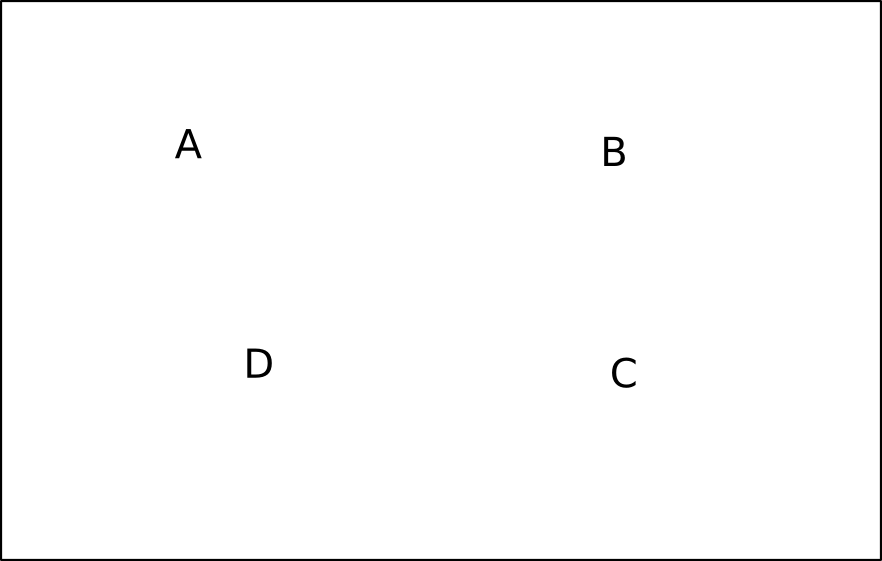
\includegraphics[scale=1.0]{"figures/michelson-morley.png"} \caption{Experimental layout of the Michelson-Morley type experiments}
\end{center}
\end{figure}

The interference pattern encodes the phase difference $ \Theta_1  - \Theta_2 $ between the Arahanov-Bohm phase changes experienced by the two beams as they travel between \textbf{A} and \textbf{C}, via the paths \textbf{ABC} and \textbf{AB'C} respectively.

Now let us assume that there exist fluxes, corresponding to the curvature $ F^I_{\mu\nu} $ of a gauge connection $ A^I_\mu $, piercing the surface bounded by the closed path \textbf{L${}_\gamma$} $ = $ \textbf{L\subsc{1}} $ \cup $ \textbf{L\subsc{2}}. Such a flux would take the form:

\begin{equation}\label{eqn:curvature_flux}
\delta \phi^I [ \mathcal{S} ] = \int_\mathcal{S} F^I_{\mu\nu} n^\mu dx^\nu 
\end{equation}

where $ I, J, K, \dots $ are Lie algebra indices, $ \mu, \nu, \dots $ are spacetime indices and $ \mathcal{S} $ denotes the surface bounded by \textbf{L${}_\gamma$}.

In the classic setup, the experimentalist employs light beams with the spin-1 photons being the corresponding excitations whose phase shifts are measured. However nothing prevents us from using any excitation we like from the particle spectrum of the standard model. Each excitation would undergo a phase shift corresponding to the flux of the connection associated with that particular excitation. For instance, electrons, muons and neutrinos would respond to the electroweak component of the flux while hadrons would respond to the strong component. If we were given some species of massless fermions which couple to the gauge group $ SU(2) $ for the gravitational connection, then their phases would measure the strength of the gravitational field in the region bounded by \textbf{L${}_\gamma$}.

For an abelian connection, such as a $ U(1) $ connection the Lie algebra is one-dimensional and its corresponding index is trivial. We have: $ F_{\mu\nu} = \partial_\mu A_\nu $, inserting this into \ref{eqn:curvature_flux} and using Stokes' theorem we find:

\begin{equation}\label{eqn:curvature_flux2}
\delta \phi [ \mathcal{S} ] = \int_\mathcal{S} \partial_\mu A_\nu n^\mu dx^\nu = \int_{L_\gamma} A(\vec{x}(\gamma))_\mu \cdot d\vec{x}(\gamma)^\mu
\end{equation}


For a non-abelian connection $ A^I_\mu $, the Lie-algebra index is non-trivial \emph{and} the expression for curvature has an additional term: $ F^I_{\mu\nu} = \partial_\mu A_\nu + g \, \epsilon^I_{JK} [ A^J_\mu, A^K_\nu ] $, where $ g $ determines the strength of the self-interactions of the gauge field. Consequently the expression for phase shift, or holonomy, becomes:

\begin{equation}\label{eqn:curvature_flux3}
\delta \phi^I [ \mathcal{S} ] = \int_\mathcal{S} \left\{ \partial_\mu A^I_\nu  + g \epsilon^I_{JK} [ A^J_\mu, A^K_\nu ] \right \} n^\mu dx^\nu = \int_{L_\gamma} A(\vec{x}(\gamma))_\mu \cdot d\vec{x}(\gamma)^\mu
	\end{equation}

\end{doublespace}




